\documentclass[a4paper,12pt]{report}

\usepackage[utf8]{inputenc}
\usepackage[T1]{fontenc}
\usepackage[french]{babel}
\usepackage{geometry}
\geometry{margin=2.5cm}
\usepackage{setspace}
\onehalfspacing
\usepackage{hyperref}
\usepackage{longtable}
\usepackage{array}
\usepackage{graphicx}
\usepackage{float}
\graphicspath{{images/}}
\makeatletter
\def\chapter{\@startsection {chapter}{0}{\z@}
                                   {-3.5ex \@plus -1ex \@minus -.2ex}
                                   {2.3ex \@plus.2ex}
                                   {\normalfont\huge\bfseries}}
\makeatother
\begin{document}

\begin{titlepage}
    \centering
    {\Huge\bfseries Projet SGBD : Gestion des Parkings du Campus \par}
    \vspace{1cm}
    {\Large 2\textsuperscript{e} année Informatique \par}
    \vfill


    \begin{figure}
        \centering
        
\includegraphics[width=0.5\linewidth]{logo_em.jpg}
        \label{fig:placeholder}
    \end{figure}

    \begin{flushleft}
{\large \textbf{Encadrant :}} \\
\vspace{0.2cm}
{\Large Nom de l'encadrant : \\ \textit{LOMBARDY} Sylvain \\ \textit{MOSABAH} Mohamed} \\ 
\end{flushleft}

\vspace{1.5cm}

\begin{flushright}
{\large \textbf{Réalisé par :}} \\
\vspace{0.3cm}
{\Large
\begin{tabular}{l}
• \textit{Anas QUATRA} \\ 
• \textit{Soufiane SBAI} \\ 
• \textit{Aymane KECHNA} \\  
• \textit{Mohamed Aziz MIGAOU}\\  
\end{tabular}
}
\end{flushright}

\vfill
{\large \today}
\end{titlepage}

\tableofcontents
\newpage

\chapter{Introduction}

\section{Contexte du projet}
Ce projet s'inscrit dans le cadre du module \textbf{Systèmes de Gestion de Bases de Données (SGBD)}. 
Il consiste à concevoir et implémenter une base de données relationnelle permettant de gérer 
les parkings du campus universitaire. 

La base doit offrir des fonctionnalités de gestion des parkings, des places, des utilisateurs, 
des véhicules, des abonnements et des stationnements, tout en permettant des consultations, 
statistiques et opérations de mise à jour.

\section{Objectifs du projet}
Le projet vise à :
\begin{itemize}
    \item modéliser les données via un MCD puis un MLD ;
    \item créer la base relationnelle sous PostgreSQL ;
    \item garantir l'intégrité et la cohérence des informations ;
    \item fournir des requêtes de consultation et de statistiques pertinentes ;
    \item permettre l'évolution du schéma pour des besoins futurs.
\end{itemize}

\chapter{Modèle conceptuel initial}

Le premier modèle conceptuel de données (MCD) proposé est présenté ci-dessous. 
Il constitue une première base de réflexion sur les entités importantes du système 
de gestion des parkings du campus.
\begin{figure}[H]
    \centering
    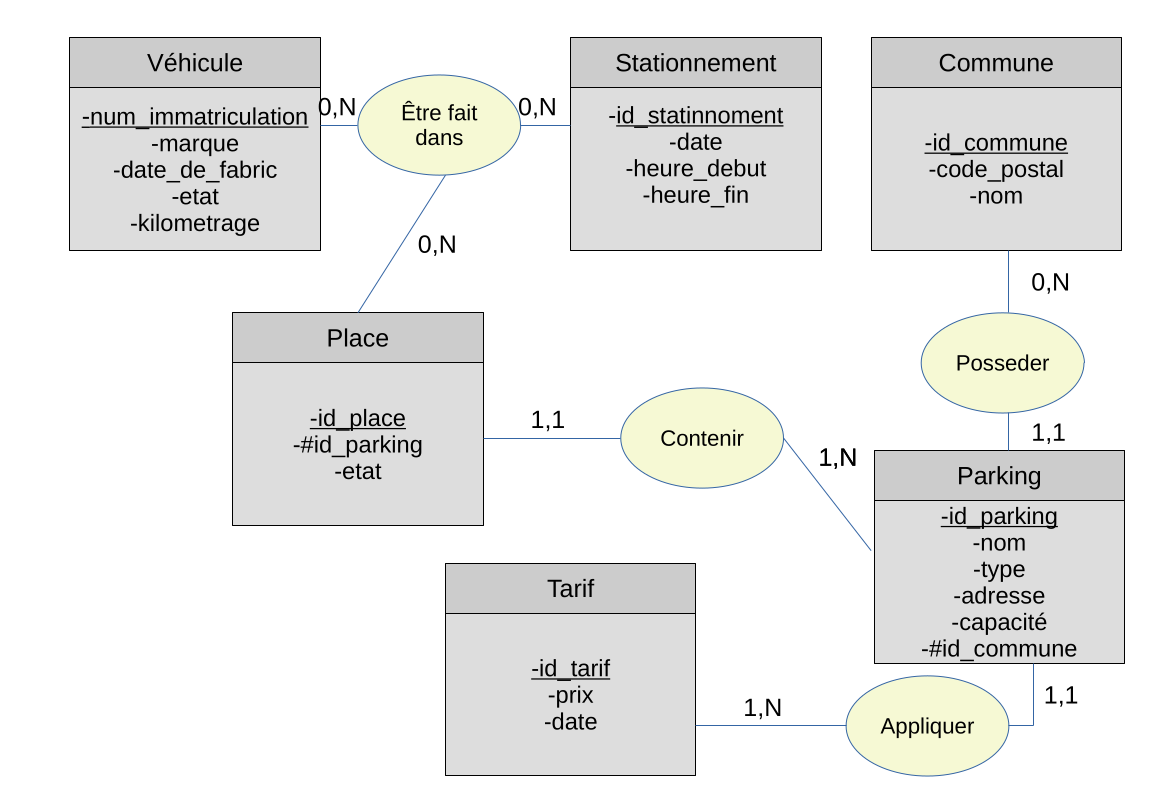
\includegraphics[width=14cm]{modele-concep-init.png}
    \caption{Modèle Conceptuel Initial du système}
\end{figure}

Ce modèle identifie cinq entités principales :
\begin{itemize}
    \item \textbf{Commune} : contient les informations de localisation (id, nom, code postal).
    \item \textbf{Parking} : décrit les parkings (id, nom, type, capacité, adresse), chacun étant situé dans une seule commune.
    \item \textbf{Place} : représente les places de stationnement d’un parking.
    \item \textbf{Véhicule} : décrit les véhicules (immatriculation, marque, état, kilométrage…).
    \item \textbf{Tarif} : correspond à un tarif appliqué à un parking ou à une place.
    \item \textbf{Stationnement} : représente les événements de stationnement d’un véhicule.
\end{itemize}

Des associations structurent ces entités :
\begin{itemize}
    \item \textbf{Contenir} : une commune contient plusieurs parkings.
    \item \textbf{Posséder} : un véhicule peut apparaître dans plusieurs stationnements.
    \item \textbf{Être fait dans} : un stationnement se déroule sur une place.
    \item \textbf{Appliquer} : un tarif est appliqué à un parking (relation floue dans ce modèle initial).
\end{itemize}

\section{Limites du modèle initial}

Bien que fonctionnel pour une première approche, ce modèle présente plusieurs limites :

\subsubsection*{1. Absence d'entités essentielles}
Le modèle initial ne prend pas en compte :
\begin{itemize}
    \item les \textbf{utilisateurs} (propriétaires de véhicules, clients du parking),
    \item les \textbf{abonnements}, pourtant très importants dans un système de gestion de parkings,
    \item les \textbf{comptes utilisateurs} (identifiant, mot de passe)
\end{itemize}

\subsubsection*{2. Relations imprécises ou insuffisantes}
\begin{itemize}
    \item La relation \textbf{Appliquer} ne précise pas à quoi le tarif s’applique (parking seul ? place ? catégorie ?).
    \item La date du tarif est insuffisante : un tarif doit définir au minimum une \textbf{plage horaire} (heure début / heure fin).
\end{itemize}

\subsubsection*{4. Problèmes d’évolution du système}
Le modèle initial ne permet pas :
\begin{itemize}
    \item de gérer plusieurs tarifs dans un même parking selon la catégorie, puisqu'il n'y a pas de notion de catégorie de place.
    \item de gérer les parkings qui proposent des abonnements.
    \item d'avoir un histroique de qui a garé dans les différents stationnements. Pour un stationnnement on ne connait que la véhicule, le temps et la place. Et s'est important d'avoir le qui.
    \item de savoir les propriétaire des différents véhicules

\end{itemize}

\chapter{Modèle amélioré}

À partir des limites discutées précédement, un modèle conceptuel amélioré a été construit. Ce modèle corrige 
les problèmes identifiés et enrichit le système pour répondre complètement aux besoins du projet.


\section{Schèma conceptuel du modèle}

Afin d’éviter toute ambiguïté lors de la modélisation, nous retenons les hypothèses suivantes :
\begin{itemize}
    \item Chaque parking est associé à une seule commune.
    \item Chaque place appartient à un unique parking et correspond à une seule catégorie.
    \item Un tarif définit de manière unique la politique de tarification pour un couple \textit{(parking, catégorie de place)}.
    \item Un tarif peut être composé d’un ou plusieurs créneaux, chacun représentant le prix horaire applicable sur un intervalle de temps donné.
    \item Un utilisateur peut garer un véhicule dont il n’est pas propriétaire.
    \item Un véhicule ou un utilisateur peut souscrire plusieurs abonnements (par exemple dans différents parkings).
    \item Un utilisateur peut utiliser le parking sans disposer d’un compte sur le site.
\end{itemize}

La figure ci-dessous représente le schèma conceptuel du modèle amélioré en tenant compte de ces hypothèses.

\begin{figure}[H]
    \centering
    \hspace*{-0.8cm}
    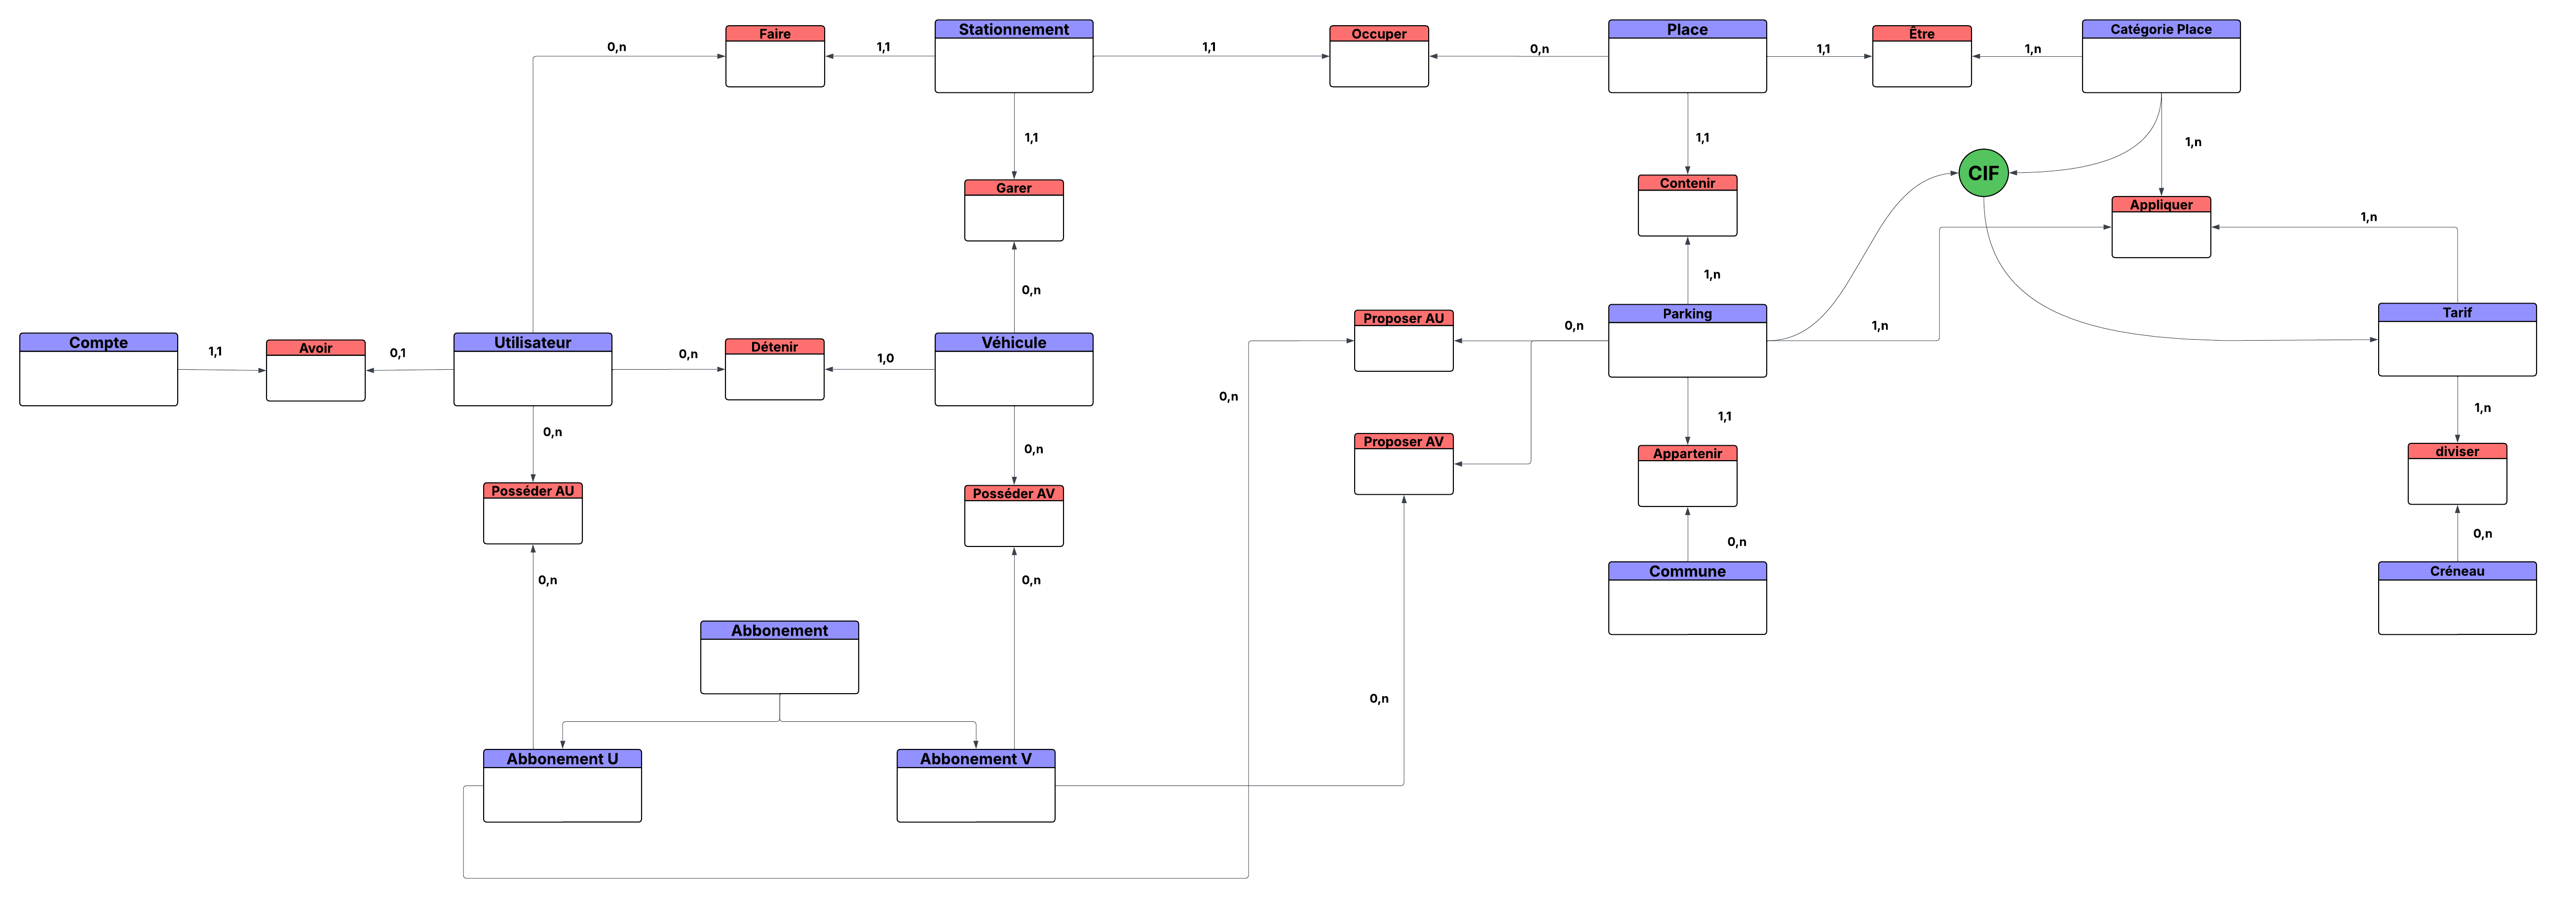
\includegraphics[width=18cm]{version-ameliore.png}
    \caption{Modèle Conceptuel Amélioré du système}
\end{figure}

\section{Schèma relationnel du modèle}

À partir du modèle conceptuel ci-dessus, le modèle relationnel a été enrichi pour mieux couvrir les besoins fonctionnels du système. Nous utiliserons les conventions suivantes :
\begin{itemize}
    \item les \textbf{clés primaires} sont \underline{soulignées} ;
    \item les \textbf{clés étrangères} sont précédées du symbole \#.
\end{itemize}

\subsection*{Schèma relationnel}

\begin{itemize}
    \item \textbf{COMMUNE}(\underline{id\_commune}, code\_postal, nom\_commune)
    
    \item \textbf{PARKING}(\underline{id\_parking}, nom\_parking, type\_parking, adresse, capacite, \#id\_commune)
    
    \item \textbf{CATEGORIE\_PLACE}(\underline{id\_categorie\_place}, type\_place)
    
    \item \textbf{PLACE}(\underline{id\_place}, num\_place, etat\_place, \#id\_parking, \#id\_categorie\_place)
    
    \item \textbf{TARIF}(\underline{id\_tarif}, prix, heure\_debut, heure\_fin)
    
    \item \textbf{APPLIQUER}(\underline{\#id\_parking, \#id\_categorie\_place, \#id\_tarif})
    \begin{itemize}
        \item clé primaire composée : (\#id\_parking, \#id\_categorie\_place, \#id\_tarif)
    \end{itemize}
    
    \item \textbf{UTILISATEUR}(\underline{id\_utilisateur}, piece\_identite)
    
    \item \textbf{COMPTE}(\underline{id\_compte}, identifiant, mot\_de\_passe, date\_creation, \#id\_utilisateur)
    
    \item \textbf{VEHICULE}(\underline{id\_vehicule}, num\_immatriculation, marque\_vehicule, date\_de\_fabrication,
    etat\_vehicule, kilometrage, \#id\_utilisateur)
    
    \item \textbf{ABONNEMENT}(\underline{id\_abonnement}, date\_debut\_abonnement, date\_fin\_abonnement,
    type\_abonnement, tarif\_mensuel\_abonnement)
    
    \item \textbf{POSSEDER\_AU}(\underline{\#id\_vehicule, \#id\_abonnement})
    
    \item \textbf{POSSEDER\_AV}(\underline{\#id\_utilisateur, \#id\_abonnement})
    
    \item \textbf{STATIONNEMENT}(\underline{id\_stationnement}, date\_debut, date\_fin, heure\_debut, heure\_fin,
    mode\_paiement, \#id\_vehicule, \#id\_place, \#id\_utilisateur)
    
    \item \textbf{CRENEAU}(\underline{id\_creneau}, prix\_horaire, tstmp\_debut, tstmp\_fin)
    \item \textbf{TARIF}(\underline{id\_tarif})
    \item \textbf{DIVISER}(\underline{\#id\_tarif \#id\_creneau})
\end{itemize}


\chapter{Évolutions du schéma entité–association : justification des choix}
\label{sec:evolutions-ee}

Cette partie présente les principales modifications apportées au modèle conceptuel initial, 
ainsi que les raisons fonctionnelles, techniques et métiers qui ont motivé ces évolutions. 
L’objectif est de disposer d’un schéma robuste, cohérent et suffisamment flexible pour 
permettre l’extension du système dans le futur.


\section{Remplacement de la relation ternaire « Être fait dans »}
\label{subsec:relation-ternaire}

Dans le modèle initial, le stationnement était représenté par une relation ternaire 
entre \textbf{Stationnement}, \textbf{Véhicule} et \textbf{Place}. Ce type de relation, 
en plus d'être ambigu, est difficile à traduire fidèlement dans un modèle relationnel 
sans perdre des contraintes importantes.

Afin de lever toute ambiguïté, la relation ternaire a été remplacée par deux associations 
binaires distinctes :

\begin{enumerate}
    \item \textbf{Stationnement -- Place} : chaque stationnement se déroule sur exactement 
    une place (1,1), tandis qu'une même place peut accueillir plusieurs stationnements 
    successifs dans le temps (0,n).

    \item \textbf{Stationnement -- Véhicule} : chaque stationnement est lié à un véhicule 
    unique (1,1), et un véhicule peut apparaître dans plusieurs stationnements (0,n).
\end{enumerate}

Cette transformation permet une modélisation plus claire des contraintes et simplifie 
la gestion en base de données : les clés étrangères sont explicites, la vérification 
de cohérence est plus simple et le modèle devient extensible (ajout de capteurs, 
historique, contrôles d’accès, etc.).


\section{Tarification : catégories de places et créneaux horaires}
\label{subsec:tarification}

Le modèle initial ne faisait pas de distinction entre les différents types de places 
(par exemple : moto, voiture, vélo, etc..). Pour rendre le système plus fidèle 
à la réalité et permettre une tarification flexible, nous introduisons l’entité 
\textbf{Catégorie de Place}. Celle-ci permet de caractériser chaque place et sert 
de base à la politique tarifaire.

De plus, la tarification peut varier selon l’heure de la journée ou d’autres critères 
temporels. Pour répondre à ce besoin, nous ajoutons l’entité \textbf{Créneau}, qui 
définit un intervalle de temps possédant un \emph{prix horaire} associé.

\paragraph{Unicité du tarif par couple (Parking, Catégorie P)}
Un point essentiel du modèle est d’imposer qu’un parking ne possède qu’un seul tarif 
par type de place. Cette règle se traduit par la dépendance fonctionnelle :

\[
(\textit{Parking}, \textit{Catégorie P}) \rightarrow \textit{Tarif}
\]

Ainsi, un \textbf{Tarif} représente la politique tarifaire globale pour un couple 
(parking, catégorie). Ce tarif est ensuite détaillé en plusieurs \textbf{Créneaux} 
qui portent les variations horaires. Cela garantit une structure claire et évite 
la duplication de tarifs incohérents dans la base.


\section{Utilisateur (identité légale) et Compte (site web)}
\label{subsec:utilisateur-compte}
\noindent \textbf{Utilisateur} : Nous avons introduit l’entité utilisateur  afin de disposer d’une représentation 
claire et stable de la personne physique. Cette entité permet notamment :
\begin{itemize}
    \item d’identifier légalement la personne responsable d’un véhicule ou d’un stationnement.
    \item de conserver des informations indépendantes de tout accès informatique (la pièce d’identité suffit dans notre cas).
    \item de gérer le cas des usagers qui utilisent le parking sans forcément disposer d’un accès en ligne.
\end{itemize}

\noindent \textbf{Compte} : Nous avons également ajouté l’entité compte, destinée à modéliser l’accès 
au site web. Elle regroupe :
\begin{itemize}
    \item l’identifiant et le mot de passe de connexion,
    \item les informations propres à l’espace client (date de création, statut),
    \item les fonctionnalités numériques offertes par la plateforme.
\end{itemize}

\vspace{5mm}

Enfin, nous avons choisi de distinguer clairement \textbf{Utilisateur} et \textbf{Compte}, 
car ils remplissent des rôles totalement différents. Cette séparation présente plusieurs avantages :
\begin{itemize}
    \item un utilisateur peut exister dans le système sans posséder de compte (ex. : visiteur occasionnel).
    \item Accès, depuis le compte web, à l’historique déjà présent dans la base, car la personne physique existe avant la création du compte et peut être facilement reliée à celui-ci.
    \item les données légales et les données numériques sont isolées, ce qui facilite la gestion et renforce la cohérence du modèle.
\end{itemize}

Cette distinction améliore donc à la fois la précision du modèle conceptuel et la flexibilité du système d’information.

\section{Distinction entre abonnements utilisateur et abonnements véhicule}
\label{subsec:abonnements}

Le modèle final distingue deux types d’abonnements, car ils correspondent à des usages 
et des modes de contrôle différents :

\begin{itemize}
    \item \textbf{Abonnement U (Utilisateur)} : l’abonné bénéficie de l’offre quel que 
    soit le véhicule qu’il utilise. Cet abonnement est contrôlé via l’identité.

    \item \textbf{Abonnement V (Véhicule)} : c’est le véhicule lui-même qui est abonné. 
    Toute personne entrant avec ce véhicule bénéficie automatiquement des avantages. 
    Ce modèle est utilisé dans le cadre de flottes ou de véhicules d’entreprise.
\end{itemize}

La présence des deux types assure une grande flexibilité opérationnelle et permet de 
modéliser fidèlement les offres commerciales réelles des parkings.

\section{Propriété des véhicules et action de stationner}

Un véhicule peut être détenu par une personne, mais garé par une autre. Pour représenter clairement ces deux aspects, nous avons introduit deux relations distinctes :

\begin{enumerate}
    \item \textbf{Relation de propriété} (\textit{Utilisateur} -- \textit{Véhicule}) : 
    elle indique à qui appartient le véhicule. Un véhicule a soit un propriétaire connu (il a utilisé le parking avec cette voiture au moins une foix), soit aucun lorsque l’information n’est pas disponible dans la base.

    \item \textbf{Relation Stationner} (\textit{Stationnement} -- \textit{Utilisateur}) : 
    elle identifie la personne qui a effectivement garé le véhicule. Cette personne peut être différente du ou des propriétaires (ex. : prêt du véhicule, voiturier, membre de la famille).
\end{enumerate}

\noindent\textit{Remarque.}  
L’information permettant de savoir si la personne qui se gare est ou non propriétaire du véhicule est supposée être recueillie au moment de l’entrée dans le parking (déclaration, badge, plaque associée à un compte, etc.).

\noindent Cette séparation améliore à la fois la précision et le niveau de couverture du modèle, et permet d’exploiter distinctement la responsabilité légale, l’usage réel du véhicule, ainsi qu’un historique plus riche des stationnements, aussi bien pour les différents conducteurs que pour les propriétaires éventuels.





\chapter{Application}
\label{sec:application}

Cette section présente la mise en œuvre pratique de l’application : création et gestion de la base PostgreSQL, conception de l’interface utilisateur et fonctionnement du serveur API, ainsi que la mise en ligne finale de l’application complète, afin de la rendre accessible publiquement via l’URL : \url{https://parking-app-521c.onrender.com}.

\section{Base locale et connexion serveur}
\label{subsec:base-locale}

On décrit ici la création d’une base PostgreSQL locale pour le développement et la configuration du serveur pour se connecter de manière sécurisée via des variables d’environnement.


\subsection{Installation et création de la base locale}
Chaque membre du groupe installe PostgreSQL sur sa machine et crée une base dédiée pour les tests.  
L’initialisation de la base se fait à l’aide des scripts fournis : \texttt{drop.sql}, \texttt{create.sql} et \texttt{insert.sql}.  
Ces scripts permettent de créer les tables puis d’insérer un jeu minimal de données de test.

\subsection{Connexion serveur - base locale}
Pour se connecter à la base depuis le serveur sans exposer les identifiants dans le code, nous utilisons des variables d’environnement stockées dans un fichier \texttt{.env}, propre à chaque machine. Ce fichier est ignoré par Git pour préserver la confidentialité.  

Un exemple de fichier \texttt{.env} est présenté ci-dessous :

\begin{verbatim}
PGHOST=localhost
PGUSER=postgres
PGPASSWORD=motdepasse
PGDATABASE=parking_local
PGPORT=5432
\end{verbatim}

Le serveur utilise ces variables pour établir la connexion avec PostgreSQL via le pool de connexions :


\begin{verbatim}
const pool = new Pool({
    user: process.env.PGUSER,
    host: process.env.PGHOST,
    database: process.env.PGDATABASE,
    password: process.env.PGPASSWORD,
    port: process.env.PGPORT,
});
\end{verbatim}

Cette approche permet de sécuriser les informations sensibles et de faciliter la configuration de chaque environnement de développement.

\chapter{Interface Utilisateur}

\section{Présentation de l'Interface}

L'interface utilisateur de notre application de gestion de parkings a été conçue pour offrir une expérience intuitive et fonctionnelle. Elle permet aux différents acteurs du système d'accéder aux données de manière sécurisée et organisée.

\subsection{Architecture de l'Interface}

L'interface est structurée en une application web qui se décompose en deux écrans principaux :

\subsubsection*{Écran de Connexion}
La première page présentée à l'utilisateur est un formulaire de connexion qui permet :
\begin{itemize}
    \item \textbf{Identification} : numéro de pièce d'identité
    \item \textbf{Authentification} : nom d'utilisateur et mot de passe
    \item \textbf{Inscription automatique} : si l'utilisateur n'existe pas, il est automatiquement créé
\end{itemize}

\subsubsection*{Tableau de Bord Principal}
Après authentification, l'utilisateur accède à un tableau de bord organisé en deux panneaux :
\begin{itemize}
    \item \textbf{Panneau latéral} : liste des requêtes disponibles avec leurs paramètres
    \item \textbf{Panneau principal} : affichage des résultats des requêtes sous forme de tableaux
\end{itemize}

\section{Flux de Communication Client-Serveur}

Le fonctionnement de l'interface repose sur une communication asynchrone entre le client (navigateur) et le serveur API. Le flux complet pour une requête typique suit une architecture REST standardisée en quatre étapes principales.

\subsubsection*{1. Interaction Utilisateur}
L'utilisateur interagit avec l'interface, par exemple en cliquant sur le bouton \texttt{"Voitures par parking"}. Le gestionnaire d'événements capture cette action et lance le processus.

\subsubsection*{2. Construction et Envoi de la Requête}
Le client construit une requête HTTP vers l'API REST du serveur :
\begin{verbatim}
GET /api/queries/voitures-par-parking
\end{verbatim}
La requête utilise la fonction JavaScript \texttt{fetch()} pour une communication asynchrone.

\subsubsection*{3. Traitement Serveur et Base de Données}
Le serveur Express.js route la requête vers le contrôleur approprié qui exécute la requête SQL correspondante sur la base PostgreSQL :

\begin{verbatim}
SELECT p.nom_parking, COUNT(v.id_vehicule) as nombre_voitures
FROM parking p
LEFT JOIN place pl ON p.id_parking = pl.id_parking
LEFT JOIN stationnement s ON pl.id_place = s.id_place
LEFT JOIN vehicule v ON s.id_vehicule = v.id_vehicule
GROUP BY p.id_parking, p.nom_parking
ORDER BY nombre_voitures DESC;
\end{verbatim}

\subsubsection*{4. Réponse et Affichage}
Le serveur retourne une réponse JSON structurée :
\begin{verbatim}
{
    "success": true,
    "data": [...],
    "timestamp": "2025-12-04T10:30:00Z"
}
\end{verbatim}
Le client reçoit cette réponse, formate les données et les affiche dans un tableau HTML dynamique.

\section{Hébergement en ligne}
\label{subsec:hebergement}

L’application est entièrement déployée en ligne pour permettre une consultation publique.

\subsection{Base de données publique}
\label{subsubsec:railway}

Pour disposer d’une base accessible en ligne, nous utilisons Railway, une plateforme cloud pour héberger des applications. Railway fournit une instance PostgreSQL managée et une chaîne de connexion \texttt{DATABASE\_URL} prête à l’emploi. La base est initialisée à l’aide des scripts \texttt{create.sql} et \texttt{insert.sql}, qui sont importés directement via l’interface Railway ou avec \texttt{psql}.

\subsection{Déploiement en ligne du serveur}
\label{subsubsec:render}

Le code de l’application est déployé sur Render, une plateforme cloud pour héberger des applications web. Les variables d’environnement sont définies directement dans le tableau de bord Render, sans fichier \texttt{.env}, en utilisant la valeur fournie par Railway (\ref{subsubsec:railway}). Render construit et exécute automatiquement le serveur API, fournit une URL publique, et reconstruit l’application à chaque mise à jour du dépôt Git, assurant un accès permanent via un lien unique.



\chapter{Conclusion}
Ce chapitre sera complété après l'implémentation, l'évaluation et les tests.

\end{document}
